\chapter{Background}\label{Background}

\section{Automatic Music Transcription}

In general, transcription refers to the process of retrieving information from audible data, such as sounds or music. Specifically within applied on music, the information we often seek is an annotation, or a transcription, of the music. Generally, transcribing a musical piece is expensive, requiring both extensive experience within a specific instrumental field as well as a lot of  time-consuming, manual work. Early on, Martin Piszczalski stated that \textit{"The learned, human skill of transcribing music is one of the most sophisticated auditory-based pattern-recognition tasks that humans perform."}~\cite{10.5555/15202}, and not long after helped introduce the term \acrfull{AMT}~\cite{piszczalski1977automatic}. Now, many years later, both the fields of \gls{AMT} and machine learning have evolved significantly.

\subsection{Transcription using Deep learning}
Currently, much of the state-of-the-art within \gls{AMT} utilizes deep learning~\cite{8350302, signals4040042, jamshidi2024machine}. With enough data, one can train a neural network to automatically, given an input sequence of music, output a transcribed sequence representing musical notation. Musical notation could be extensive in their information, but by far the most important parts could be reduced down to \textit{"which instruments are playing"} and \textit{"when are they playing"}.

Relating this to a common deep learning task, this could be described as a multi-label sequence tagging/sequence labelling task. For each element in an input sequence, output a respective one or more labels.

\begin{figure}[H]
    \centering
    \begin{tikzpicture}

\node[
    label=north:{\large{Music}}
] (music) at (-5.5, 0) {
    \begin{tikzpicture}
        \node at (0, 0) {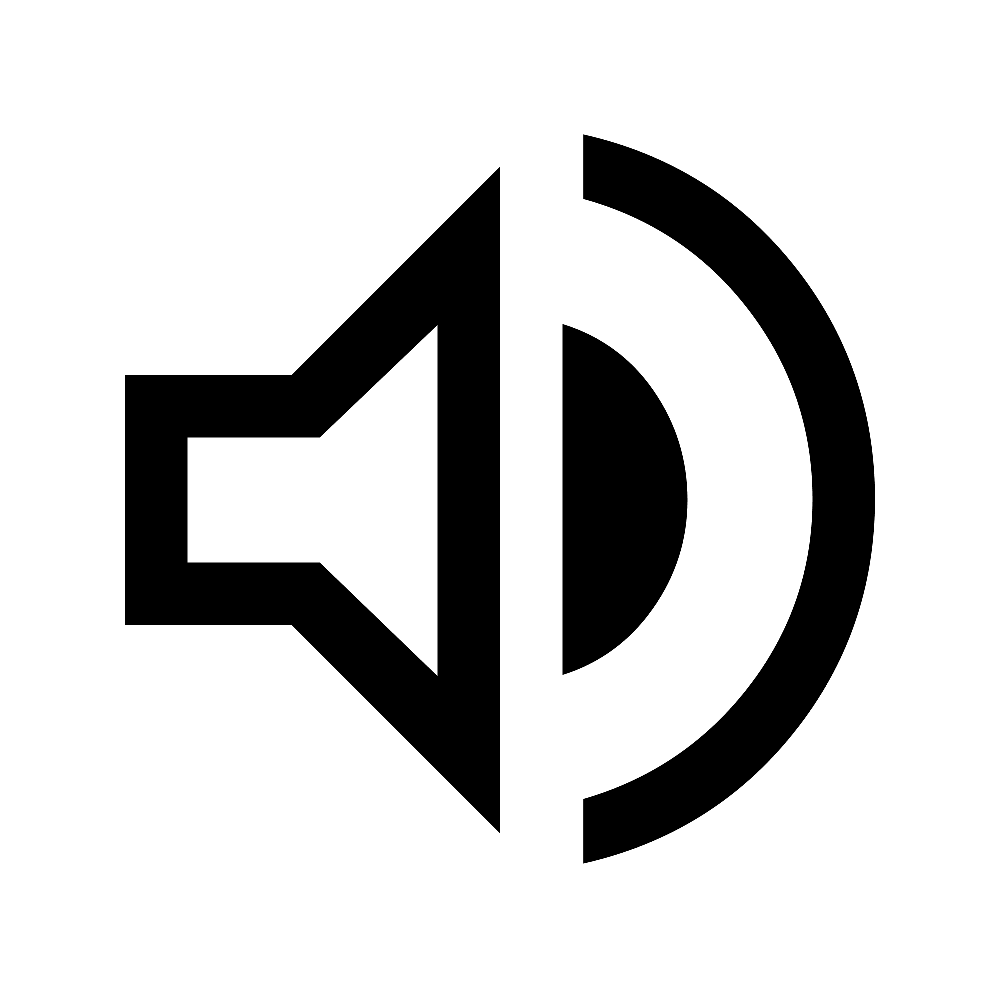
\includegraphics[scale=0.06]{figures/speaker.png}};
        \node [rotate=30, scale=1.6] at (1.1, 0.85) {\AAcht};
        \node [rotate=-30, scale=1.2] at (1, -0.75) {\Acht};
    \end{tikzpicture}
    };

\node[
    label={[label distance=1.08em]north:{\large{Deep Learning}}},
    rectangle,
    draw,
    thick,
    minimum height=5em,
    minimum width=10em,
] (nn) at (0, 0) {\large{Neural Network}};

\node[
    label={[label distance=1.08em]north:{\large{Transcription}}},
    minimum height=5em,
] (transcription) at (5.5, 0) {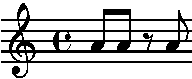
\includegraphics[scale=1.0]{lilypond/amt.cropped.pdf}};

\draw[->, thick] (music.east) -- (nn.west);
\draw[->, thick] (nn.east) -- (transcription.west);

\end{tikzpicture}

    \caption{An abstract visualization of the \acrfull{AMT} process using deep learning. Music is input into a deep learning pipeline, e.g. a neural network, which processes it, and returns a finished transcription.}
    \label{AMTFigure}
\end{figure}

\section{Audio}

Sound has be described as \textit{"the sensation caused in the nervous system by vibration of the delicate membranes of the ear."}~\cite{1953fundamentals}. In short, sound is the human perception of acoustic waves in a transition medium, like air. These waves, consisting of vibrating molecules, get sensed by our auditory organs and perceived by the brain. 

Thus sound can be described as the propogation and perception of waves. Mathematically, waves can be studied as signals~\cite{8454362}. To represent these sounds digitally, as \textit{audio}, one can express these waves as a signal, giving rise to the \textit{waveform}. The waveform is a representation of a signal as a graph, and charts the amplitude, or strength of the signal, over time.

\begin{figure}[H]
    \centering
    %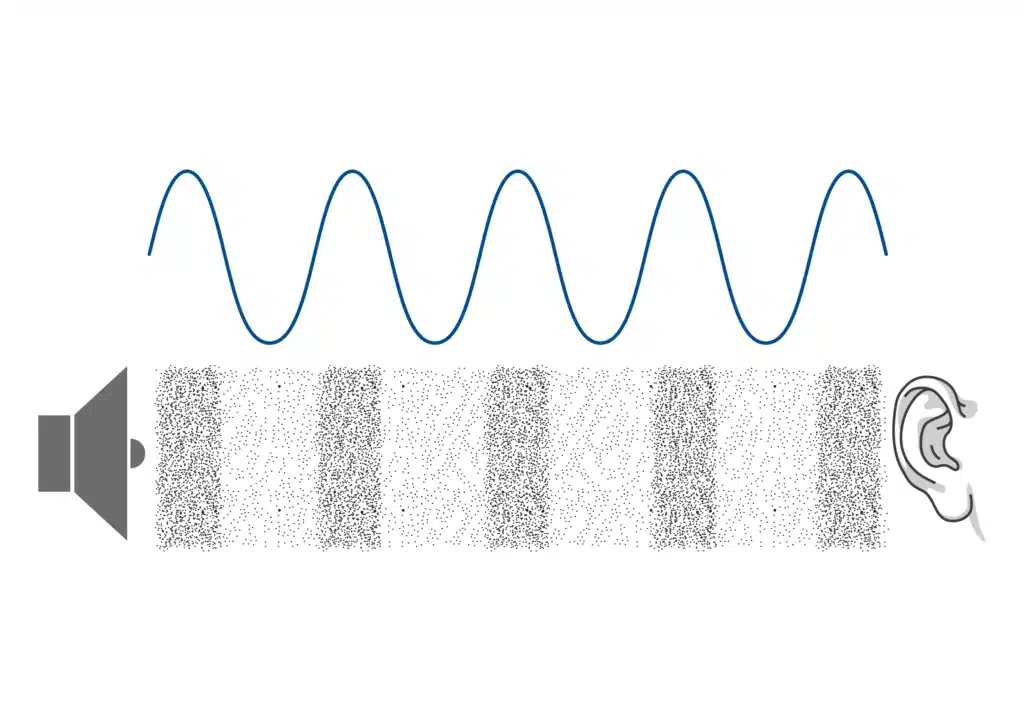
\includegraphics[scale=0.35]{figures/waveform}
    \begin{tikzpicture}

% Waveform signal
\draw[
domain=0:9, 
samples=300,
smooth,
variable=\x,
blue,
ultra thick,
shift={(-4.5, 2.2)},
] plot ({\x},{sin((3.05*\x + 0.3) r) * 0.8});
\node at (0, 3.5) {\large Digital Waveform};
    
% Pressure wave
\node[
    label=south:{\large Acoustic Sound Wave}
] (pressure) at (0, 0) {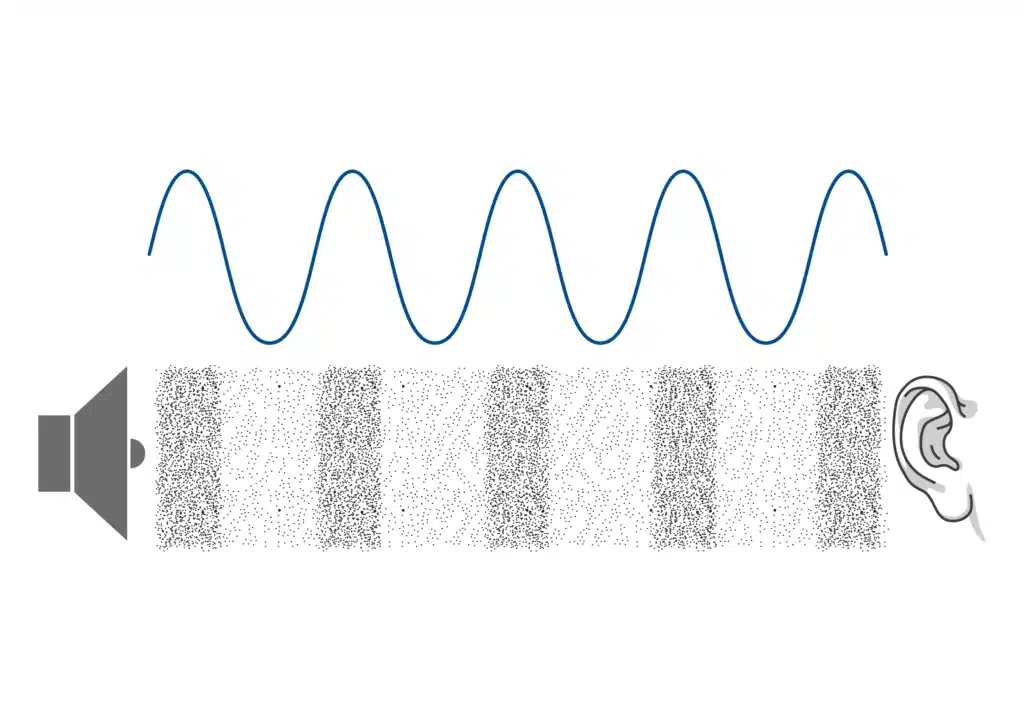
\includegraphics[trim={5.25cm 5.5cm 4.75cm 12.5cm},clip,scale=0.35]{figures/waveform}};

% Speaker
\node[left=-0.25cm of pressure] {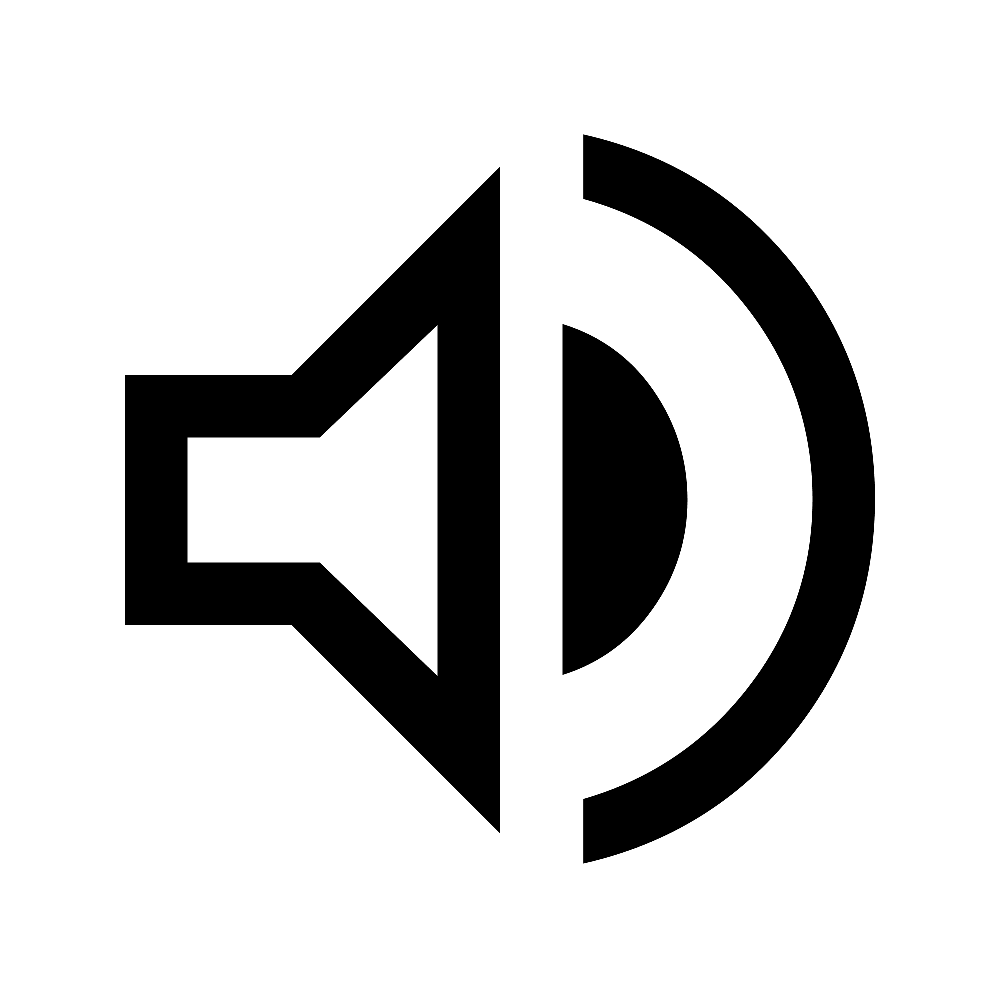
\includegraphics[scale=0.065]{figures/speaker.png}};

% Ear
\node[right=-0.25cm of pressure] {\scalebox{-1}[1]{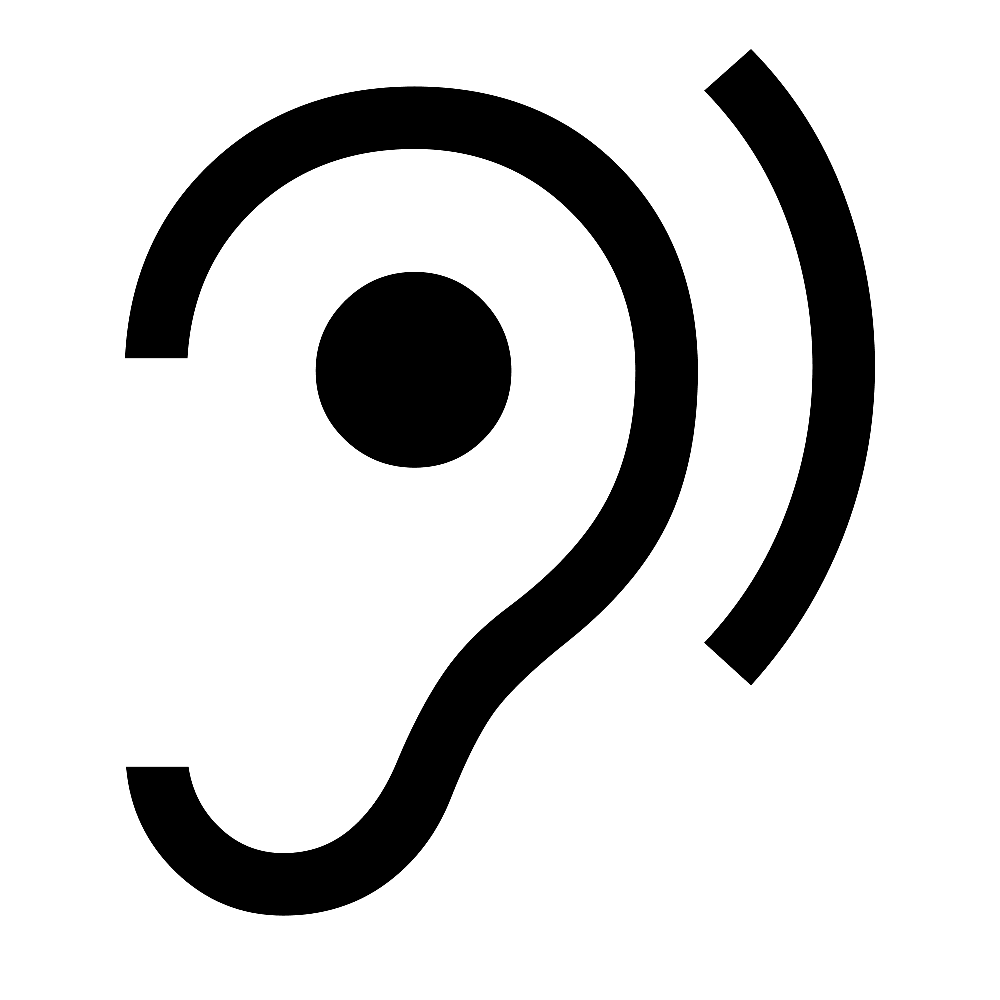
\includegraphics[scale=0.065]{figures/ear.png}}};

\end{tikzpicture}
    \caption{The sound wave to waveform relationship. The waveform represents the pressure of the air molecules in the sound wave at a given time. Higher and lower pressure in the sound waves gives respective \textit{peaks} and \textit{troughs} in the waveform.}
    \label{WaveformFigure}
\end{figure}

For monophonic sound, this waveform is a one-dimensional representation. Even though this is an excellent way of storing audio digitally, it is very compact. There have been deep learning models working directly with these waveforms, e.g. Oord et al.'s WaveNet~\cite{oord2016wavenetgenerativemodelraw}, however the task of parsing and perceiving such a signal is a complex one.

\subsection{Fourier Transform}

The Fourier Transform is a mathematical transformation which, given a frequency, computes its significance, or intensity, in a given signal. As we've established, audio is represented as a signal, and we can therefore use this transform to turn this audio signal into frequency space. 

The fourier transform is a complex transformation. Given a signal $f$, we can compute the integral \[ \widehat{f}(\xi) = \int^{\infty}_{-\infty}{f(x)e^{-i2\pi \xi x} dx} \] for a frequency $\xi \in \mathbb{R}$, computed over all values $x \in \mathbb{R}$ representing time, resulting in a \textit{complex} number on the form $\widehat{f}(\xi) = a + bi$. This number consists of a \textit{real} part $a$ and an \textit{imaginary} part $b$. We can represent this complex number in polar form \[ a + bi = re^{i\theta}, \] where $r = \sqrt{a^2 + b^2}$ denotes the magnitude (amplitude) and $\theta = \arctan{|\frac{b}{a}|}$ the phase of the respective frequency in the original signal $f$. This information is what allows us to, for a given signal, figure out which frequencies it is made out of and how much each frequency contributes. 

By doing such a transform, we turn our temporal data into spectral data. This initively \textit{untangles} our signal into its respective base frequencies. Such an transformation could lessen the complexity of the task, making \textit{understanding} of audio easier.

\begin{figure}[H]
    \centering
    \hspace*{-1.3cm}
    \begin{tikzpicture}
        \node at (0, 0) {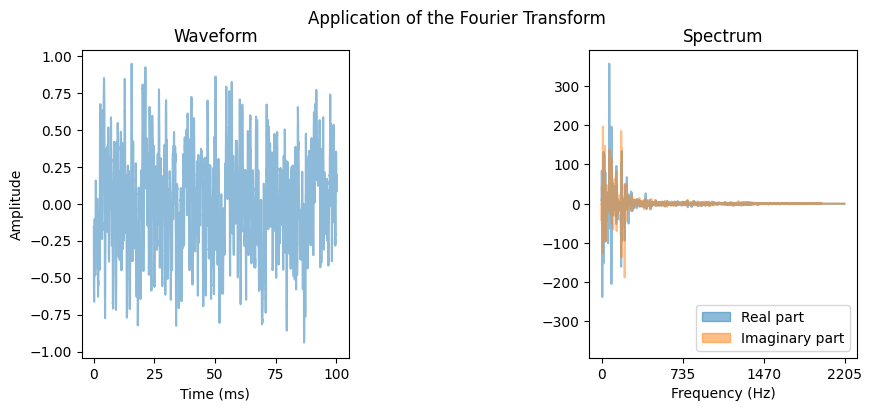
\includegraphics[scale=0.8]{figures/fouriertransform}};
        \draw[->] (-1, 0) -- (1.75, 0) node[above, midway, font=\footnotesize] {Fourier Transform};
    \end{tikzpicture}
    \caption{Applying the Fourier Transform deconstructs a wave into its respective frequency components. The waveform on the left (time-domain) is measured in amplitude, where a high amplitude denotes a high pressure level. The spectrum on the right (frequency-domain) is also measured in amplitude, but represents the strength of different frequencies in the original signal.}
    \label{FTFigure}
\end{figure}

Note that the Fourier Transform is invertible, meaning that, given information about each frequency, we can perform a similar integral and reconstruct the original signal. In signal processing, this property is exploited heavily.

\subsection{Discrete Fourier Transform}

The Fourier Transform is defined as an integral over continuous time. On computers, instead of storing signals continuously we store signals using a discrete number of samples. Each signal's \textit{sampling rate} describes how many samples a signal contains per second of audio, and is denoted in \textit{Hz}.

To extract frequency values from these signals, we instead have to use the \gls{DFT}. Intuitively this works as the normal Fourier Transform, but ported to work on discrete-valued signals. It is given by the formula \[ X_k = \sum^{N - 1}_{n=0}{x_n \cdot e^{-i 2\pi \frac{k}{N} n}}, \] where $k$ denotes a certain frequency bin and $N$ the number of discrete samples. Note that contrary to the normal Fourier transformer, instead of computing the magnitude of each specific real-valued frequency, we instead compute the magnitude of frequencies covered by certain frequency bins. The number of these bins are directly dependent on the number of samples $N$, and the respective frequencies covered by each bin is given by the signal's sampling rate.

\subsection{Nyquist frequency}

When we discretize a signal, e.g. when going from continuous audio waves in the air to discrete audio signals on a computer, we could lose some information. The discrete representation of the signal is an \textit{approximation} which quality is directly dependent on the sampling rate. The higher the sampling rate, the \textit{closer} we are to the original, continuous signal. However a higher sampling rate comes at the cost of needing to store these signals at a higher precision. A lower sampling rate would need less information stored, but this could also mean a less precise signal approxmation.

\textit{Aliasing} is the phenomena where new frequencies seem to emerge in undersampled signals. For a given discrete signal, the \textit{Nyquist frequency}, equal to half the sampling rate, is the maximum frequency a signal accurately can represent. Thus to prevent aliasing, one would need to store a signal with a sampling rate of at least double the maximum frequency.

\begin{figure}[H]
    \centering
    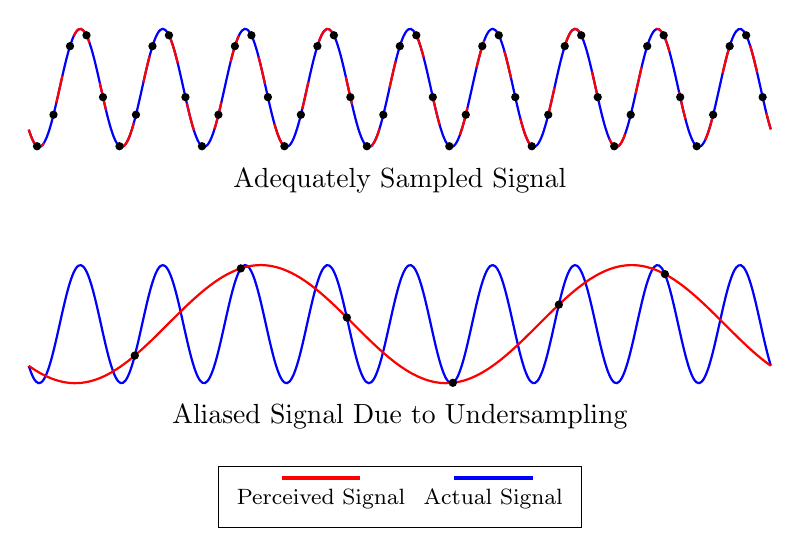
\begin{tikzpicture}[scale=1.5]

% Above Signal
\draw[
domain=0:2*pi, 
samples=300,
smooth,
variable=\x,
blue,
thick,
shift={(0, 2)}
] plot ({\x},{sin((9*\x - 3*pi/4) r)/2});

% Above Perceived
\draw[
domain=0:2*pi, 
samples=300,
smooth,
variable=\x,
red,
thick,
dash pattern={on 10pt off 15pt},
shift={(0, 2)}
] plot ({\x},{sin((9*\x - 3*pi/4) r)/2});

% Scatter Adequate Samples
\foreach \i in {1,...,45} {
    \pgfmathsetmacro\xsamp{2*pi*(\i-0.5)/45}
    \pgfmathsetmacro\ysamp{sin((9*\xsamp - 3*pi/4) r)/2}
    \fill (\xsamp, \ysamp + 2) circle (1pt);
}

% Above Text
\node[
anchor=north, 
] at (pi, 1.4) {Adequately Sampled Signal};


% Below Signal
\draw[
domain=0:2*pi, 
samples=300,
smooth,
variable=\x,
blue,
thick
] plot ({\x},{sin((9*\x - 3*pi/4) r)/2});

% Below Perceived
\draw[
domain=0:2*pi, 
samples=100,
smooth,
variable=\x,
red,
thick
] plot ({\x},{sin((2*\x - 3*pi/4) r)/2});

% Scatter Aliasing Samples
\foreach \i in {1,...,6} {
    \pgfmathsetmacro\xsamp{2*pi*\i/7}
    \pgfmathsetmacro\ysamp{sin((9*\xsamp - 3*pi/4) r)/2}
    \fill (\xsamp, \ysamp) circle (1pt);
}

% Below Text
\node[
anchor=north, 
] at (pi, -0.6) {Aliased Signal Due to Undersampling};


% Legend
\tikzset{
    legend entry/.pic={
        \draw[pic actions, line width=1.5pt] (-0.5, 0) -- (0.5, 0);
    }
}
\matrix [draw, below] at (pi, -1.2) {
    \pic[red]{legend entry}; &  \pic[blue]{legend entry}; \\
    \node[font=\footnotesize] {Perceived Signal}; &  \node[font=\footnotesize] {Actual Signal}; \\
};

\end{tikzpicture}
    \caption{Example of aliasing in an undersampled signal. The original signal has a frequency of 9Hz. Above, when sampled at a sufficient sampling rate of 45Hz we perceive the signal at its actual frequency. However below, when sampled with a sampling rate of 7Hz, we instead incorrectly perceive the signal as having a frequency of 2Hz.}
    \label{AliasingFigure}
\end{figure}

Regarding the \gls{DFT}, it here directly follows that the maximum frequency we accurately could extract information about is proportional to the sampling rate of the signal, that being it is equal to the nyquist frequency of the signal.

\subsection{Fast Fourier Transform}

Keen-eyed computer scientists may have spotted that the \gls{DFT} runs in $\mathcal{O}(n^2)$ time as we, for every frequency in the range $[0, N]$ have to sum over $N$ different values. In other words, the \gls{DFT} algorithm scales quite poorly. Take into account that the standard sampling rate for audio is $44.1 \text{kHz}$, i.e. $44100 \text{Hz}$, then we can see that the \gls{DFT} could be inefficient.~\cite{pras2010sampling}

The \gls{FFT} is an algorithm which solves this problem, and instead computes the \gls{DFT} of a signal within $\mathcal{O}(n\log{n})$ time. Described by Gilbert Strang as \textit{"the most important numerical algorithm of our lifetime"}~\cite{strang1993wavelet}, this practically solves our scaling problem, and allows us to efficiently extract spectral information from a signal regardless of sampling rate.

There exist many different implementations of the \gls{FFT}. However the Cooley-Tukey algorithm is by far the most used \gls{FFT} and optimizes calculations through a \textit{divide and conquer} approach, utilizing prior calculations to compute others.~\cite{d3ea2d52-5ab2-3128-8b80-efb85267295d}

\subsection{Short-time Fourier Transform}

The Fourier Transform comes with some drawbacks, notably how by moving from time space into frequency space, we lose temporal information. For certain tasks this might be sufficient, but the temporal dimension is vital when working with transcriptions and \gls{ADT} tasks. We've seen how the Fourier Transform computes the frequencies of a signal, but what happens if we had applied the same transform to smaller, \textit{partitions} of a signal.

This leads us to the \gls{STFT}. By instead of transforming the whole signal, we transform smaller \textit{windows}, we could gain insight into the frequency space while keeping temporal information relatively intact. This turns our data from being one-dimensional into two-dimensional, giving us insight into the intensities of different frequencies, along different timesteps.

\begin{figure}[H]
    \centering
    %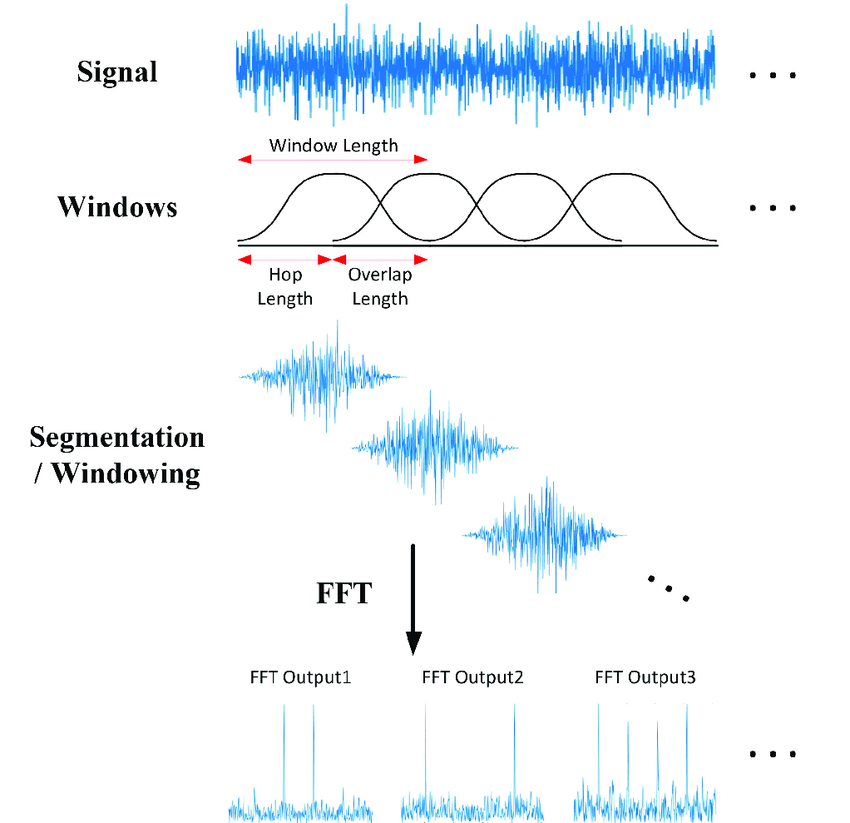
\includegraphics[scale=0.4]{figures/stft}
    \begin{tikzpicture}

% Signal
\node[
    %label=north:{\Large{Application of the Short-Time Fourier Transform}},
    label=east:{\Huge{\textbf{\dots}}},
    label={[label distance=0.6cm]west:{\large{Signal}}}
] (signal) at (0, 0) {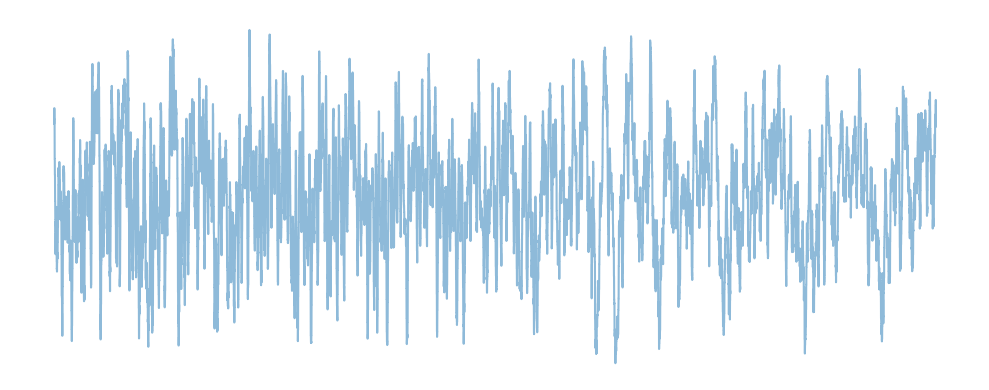
\includegraphics[scale=0.42]{figures/stftfull}};


% Window
\node[
    label=east:{\Huge{\textbf{\dots}}},
    label=west:{\large{Windows}},
    below=0.3cm of signal,
    xshift=-0.2cm
] (windows) {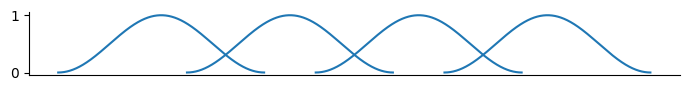
\includegraphics[scale=0.62,trim={0 0.25cm 0 0.2cm},clip]{figures/stftwindows}};

% Window Arrows
\draw[<->] ($(windows.north west) + (1.05, 0)$) -- ($(windows.north) - (1.25, 0)$) 
node[above, midway] (windowlabel) {\footnotesize{Window Length}};
\draw[<->] ($(windows.south west) + (1.05, 0)$) -- ($(windows.south) - (2.5, 0)$) 
node[below, midway] {\footnotesize{Hop Length}};


% Windows
\node[
    below=2cm of windowlabel
] (window0) {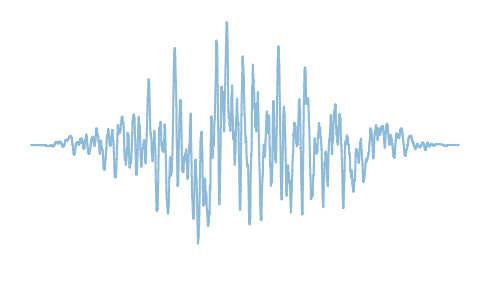
\includegraphics[scale=0.35]{figures/stftwindow0}};
\node[
    below right=-1.75cm and -1.8cm of window0,
    label={[label distance=3cm]west:{\parbox{2.5cm}{\centering \large{Window \\ Partitioning}}}}
] (window1) {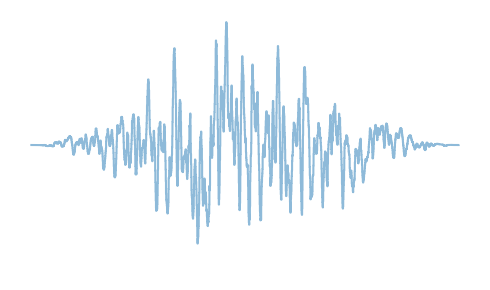
\includegraphics[scale=0.35]{figures/stftwindow1}};
\node[
    below right=-1.75cm and -1.8cm of window1,
    label={[rotate=-45]south east:{\Huge{\textbf{\dots}}}}
] (window2) {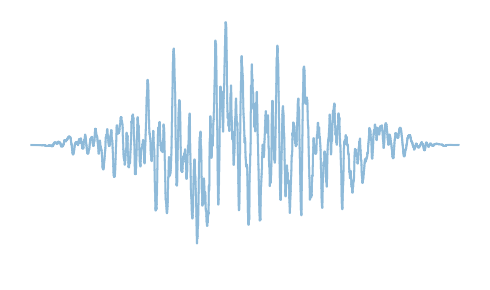
\includegraphics[scale=0.35]{figures/stftwindow2}};


% FFTs
\coordinate (fftarrow) at ($(window1.west |- window2.north) + (0, -1)$);
\draw[->, thick] (fftarrow) -- ($(fftarrow) + (0, -2.45)$) node[left, midway] {\large{FFT}};

\node[
    label=east:{\Huge{\textbf{\dots}}},
    below=1.25cm of window2,
    label={[label distance=-0.25cm]north:{\footnotesize{FFT Output 3}}}
] (fft2) {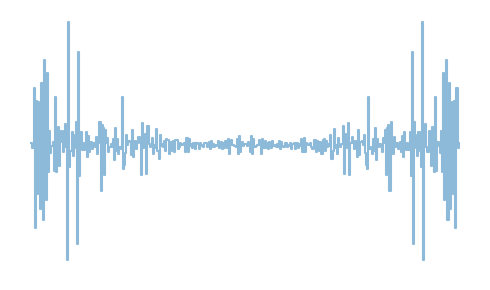
\includegraphics[scale=0.2]{figures/stft2}};
\node[
    left=0.15cm of fft2,
    label={[label distance=-0.25cm]north:{\footnotesize{FFT Output 2}}}
] (fft1) {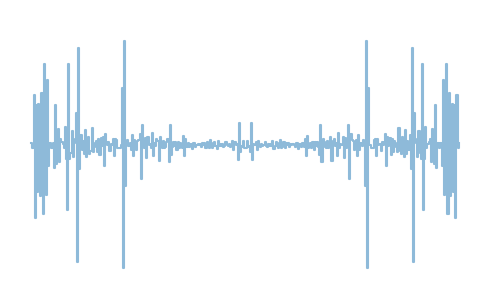
\includegraphics[scale=0.2]{figures/stft1}};
\node[
    left=0.15cm of fft1,
    label={[label distance=-0.25cm]north:{\footnotesize{FFT Output 1}}},
    label={[label distance=0.82cm]west:{\parbox{2.5cm}{\centering \large{Frequency \\ Spectra}}}}
] (fft0) {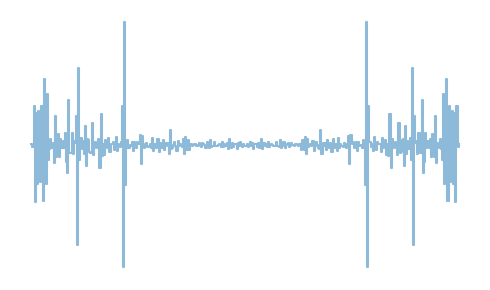
\includegraphics[scale=0.2]{figures/stft0}};

\end{tikzpicture}
    \caption{The application of the \gls{STFT} on a signal. We partition the original signal into different signal windows by multiplying it with multiple, differently offset window functions. We apply the \gls{FFT} on each of these signal partitions seperately to obtain several frequency spectra.}
    \label{STFTFigure}
\end{figure}

The \gls{STFT} comes with several parameters which affect the output format, most importantly the \textit{window function}, \textit{window length} and \textit{hop length}. Due to a phenomena called \textit{spectral leakage}, where spectral information spread larger than a window bleeds into other frequencies, a windowing function is applied per window. A usual function for this is the "Hann window", as seen in figure \ref{HannWindowFigure}. The window length is crucial regarding the time-frequency resolution, where a larger window length provides better frequency resolution, but a worse time resolution. This because it decides how much of the original signal each window \gls{FFT} should cover. By making each window larger, one is able to more accurately compute each frequency's magnitudes, but this comes at the cost of covering and overlapping more with other windows. Intuitively, smaller windows blur frequential information where as larger windows blur temporal information; a tradeoff described as the \textit{time-frequency tradeoff}. The last, hop length, also affects the temporal resolution, by deciding how many windows the signal should be partitioned into. This can also be used to give each window a temporal index. By using a lower hop length, each window would represent a smaller time window, but would require a higher number of \glspl{FFT} due to increasing the number of windows.

\begin{figure}[H]
    \centering
    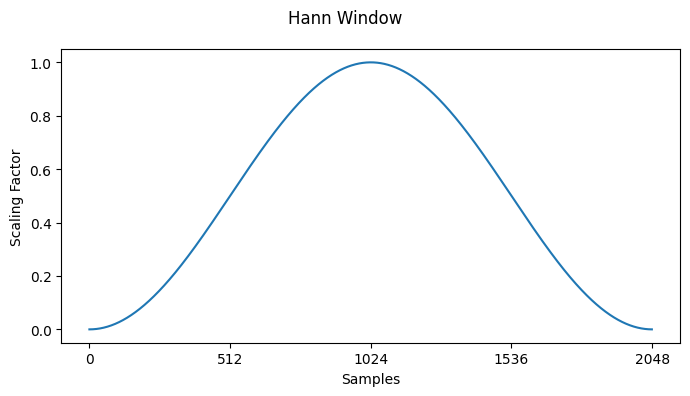
\includegraphics[scale=0.8]{figures/hann}
    \caption{The Hann window function, a function applied to each partition during the \gls{STFT} to lessen the effects of spectral leakage. It achieves this by scaling the amplitude of a partition's signal down towards the edges. This window has a window length of 2048 samples.}
    \label{HannWindowFigure}
\end{figure}

For \gls{ADT}, a common approach is to use the previously mentioned Hann-window, along with a window size of 2048 input samples, and a hop length representing 10ms, equal to the sampling rate divided by 100~\cite{8350302, vogl2016recurrent,vogl2018multiinstrumentdrumtranscription, signals4040042}.

\subsection{Spectrogram}

The \gls{STFT}, similar to the standard Fourier Transform, returns the data as complex values. To turn these into strictly real values without discarding data we can compute the spectrogram. Simply, a magnitudal spectrogram is computed by taking the absolute of each complex value from the \gls{STFT}.

This results in a 2-dimensional, real representation of our signal. A representation like this is equivalent to an \textit{image}, but can also still be modelled as a time series. In this way, we've converted our audible information into visual information. Naturally, these spectrograms can be visualized using e.g. a heatmap.

\begin{figure}[H]
    \centering
    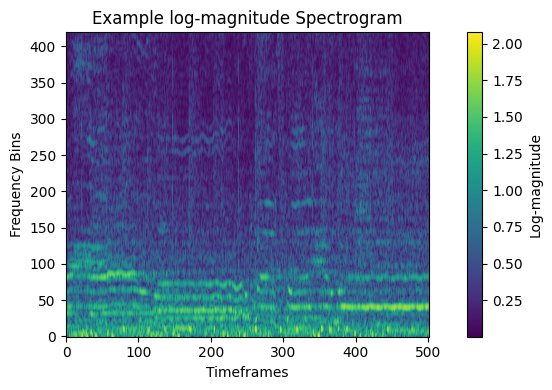
\includegraphics[scale=1.1]{figures/logspectrogram}
    \caption{Heatmap of an audio spectrogram, of the SADTP track "Red Swan" from 3:35 to 3:40 minutes. It is computed using 2048 \glspl{FFT}, with a window length of 512 and hop length representing 10ms, but with only the first 420 frequency bins being visualized. The color is represented in log-magnitude.}
    \label{SpectrogramFigure}
\end{figure}

The number of frequency bins (observed as the y-axis of Figure \ref{SpectrogramFigure}) one is left with in a spectrogram is equal to half the number of \glspl{FFT} used when computing it. These frequency bins contain frequential information about each linearly spaced frequency, from 0Hz up to the Nyquist frequency of the signal. The number of timeframes (the x-axis) is as mentioned given by the hop length of the \gls{STFT}, with a smaller hop length resulting in a larger number of timeframes. In such a way, one has significant control over the dimensionality of the spectrogram based on the values of the specific parameters. 

One drawback about the spectrogram is that it contains no information about the phase of the signal it represents. As mentioned, the phase of a signal is stored in the rotation angle of a complex number, which is discarded when taking the absolute value. That means it will not be possible to reverse the spectrogram transformartion process and recreate the exact original signal. However, one could approximate it using an algorithm like Griffin-Lim~\cite{1164317}.

\subsection{Loudness of Magnitude}

Similarly to perception of pitch, loudness also perceived an approximately logarithmic. A soundwave which is 10 times louder in energy is not perceived as being 10 times louder by us. Instead, a doubling in perceived loudness corresponds to a rougly 10 \gls{dB} increase in signal amplitude. The \acrlong{dB} is a relative unit of measurement, expressing the ratio of the power between two signals, where 1 \gls{dB} have a power ratio of $10^\frac{1}{10}$, with the power of a signal is being computed as the magnitude squared. This has two major consequences. Firstly, the magnitude scale does not follow the natural perceived loudness scale of us humans. A loud signal and a quiet signal could differ significantly in magnitude. However secondly, this means the normal spectrogram is very variational when it comes to magnitudal information, and makes it hard to identify frequencies other than the largest ones.

This is often solved by instead computing a log-magnitude spectrogram (like in Figure \ref{SpectrogramFigure}), which turns the magnitude into logarithmic scale. The base chosen for this logarithm is almost exclusively base 10, due to the \acrlong{dB} being a logarithmic scale in this scale.

\begin{figure}[H]
    \centering
    \hspace*{-1.0cm}
    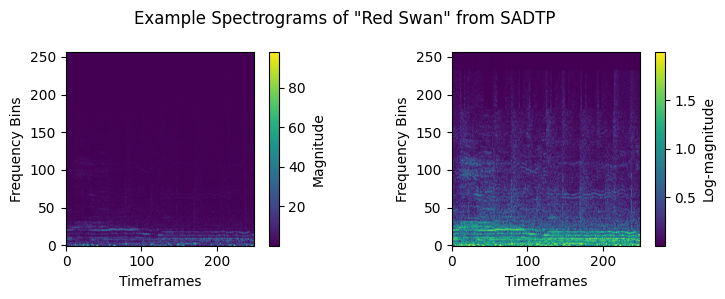
\includegraphics[scale=1.0]{figures/spectrogramlogspectrogram}
    \caption{Comparison of a magnitude spectrogram on the left with a log-magnitude spectrogram on the right. Visually, differences in magnitude are much harder to spot when scaled linearly versus when scaled logarithmically.}
    \label{SpectrogramLogspectrogramFigure}
\end{figure}

\subsection{Filters}

Signal frequencies and human perception have a special relationship. We humans percieve logarithmic differences in frequencies as a linear difference in pitch, and we tend to be better at distinguishing differences in lower frequencies than higher. E.g., the notes $\text{A}_2$ and $\text{B}_2$ have the same perceptual pitch difference as $\text{D}_7$ and $\text{E}_7$, even though their difference in frequency, $\text{B}_2 - \text{A}_2 \approx 13.471 \text{Hz}$ and $\text{E}_7 - \text{D}_7 \approx 287.703 \text{Hz}$, are vastly different. As the frequency bins in a spectrogram are linearly spaced, this leads to the spectrogram not representing each frequency equally compared to our perception.

To solve this, we can filter the spectrogram into different bins, more suited to represent our perception of sound. This filtering is done by matrix multiplying our spectrogram with a \textit{filterbank}; a matrix representation of different filters. By choosing how many filters we use in a single filterbank we have control over the number of frequency bins which remain in the resulting filtered spectrogram.

\subsubsection{Mel Spectrograms}

The mel scale, presented by Stevens, Volkmann, and Newmann in 1937, is a transformation from the frequency scale to the mel scale. These mels have the property such that a linear difference in mels are humanly percieved as linear differences in pitch. Application of mel-filters result in the \textit{mel spectrogram}, and are widely used when dealing with audio in machine learning, and successful applications have been seen in \gls{AMT}.~\cite{wolfmonheim2024spectralrhythmfeaturesaudio, gardner2022mt3multitaskmultitrackmusic, chang2024yourmt3+, 8350302, gong2021astaudiospectrogramtransformer, zehren2024analyzingreducingsynthetictorealtransfer}

\subsubsection{Logarithmic Filters}

The mel scale was created to mimic human perception of sound, however within \gls{ADT} there is a different trend. By instead using other logarithmically spaced filters, centered on the note $\text{A}_4$, we get what we in this thesis call a \textit{logarithmically filtered spectrogram}. Intuitively one could assume that this, instead of mimicing human perception, ports the spectrogram into a format preserving musical relationship and information. This seems to be a standard for \gls{ADT} and has been used extensively by the likes of Vogl et al.~\cite{Vogl2017DrumTV, vogl2018multiinstrumentdrumtranscription} Specifically, one constructs 12 different logarithmically spaced filters per octave (chosen as there exists 12 semitones in an octave), for a frequency range from 20 to 20,000 Hz (spanning the human hearing range). These filters are area-normalized, meaning each triangular filter is scaled such that the area under the curve equals 1. This results in a spectrogram with $D_{STFT} = 84$ frequency bins~\cite{8350302, signals4040042}.

\begin{figure}[H]
    \centering
    \hspace*{-0.6cm}
    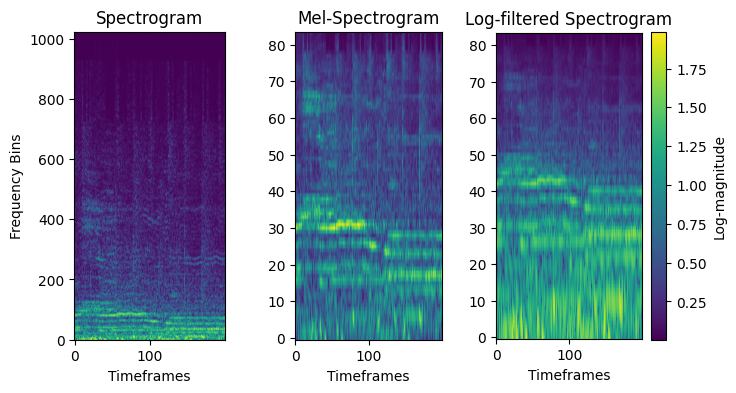
\includegraphics[scale=0.9]{figures/allspectrograms}
    \caption{Comparison between the full, log-magnitude spectrogram, with a log-magnitude mel-spectrogram and log-magnitude, log-filtered spectrogram. Both the mel-spectrogram and log-filtered spectrogram have 84 area-normalized filters. The logarithmic scaling of frequencies in the mel- and log-filtered spectrograms are observable, and frequency information is significantly more densely uniform along the vertical axis.}
    \label{AllSpectrogramFigure}
\end{figure}


\section{Transcription}

Transcription refers to a process in which we convert information from an audible format, like music, to another medium. This medium then contains a \textit{description} of said audio. As we focus on a musical context, there are a few notable such mediums.

\subsection{Music Notation}

Modern staff notation is a written transcription for a given instrument, that contains the \textit{recipe} for a musician to play parts of the original recording. This has become the standard way of noting down music, and is used by musicians of many different genres all throughout the world.

Sheet music with this notation is typically descriptively exhaustive, and contain information about musical properties like instrument onsets, tempo, velocity, etc. When reading it, time moves horizontally from left-to-right. Each note represents an onset, where the onset's pitch (for melodic instruments) or percussion (for percussive instruments, like the drum set) is denoted by the note's vertical position. The duration or time segment of a given onset is denoted by the form of the note-head or note-stem.

\begin{figure}[H]
    \centering
    \begin{tikzpicture}

\node[anchor=west] at (0, 0) {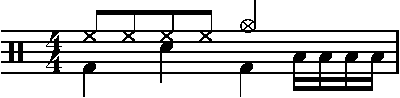
\includegraphics[scale=1.9]{lilypond/drumsheet.cropped.pdf}};

\matrix[
anchor=east,
row sep=-0.205cm
] at (0, 0.1){
    \node[font=\normalsize] {\acrshort{CC+RC}}; \\
    \node[font=\normalsize] {\acrshort{HH}}; \\
    \node[font=\normalsize] {\acrshort{SD}}; \\
    \node[font=\normalsize] {\acrshort{TT}}; \\
    \node[font=\normalsize] {\acrshort{KD}}; \\
};

\end{tikzpicture}
    \caption{An example drum sheet containing all instruments of a 5-instrument \gls{ADT} task. The instrument in each respective row is shown on the left. From the bottom they are the \acrfull{KD}, \acrfull{TT}, \acrfull{SD}, \acrfull{HH}, and \acrfull{CC+RC}.}
    \label{DrumsheetFigure}
\end{figure}

Note that rest marks, like \HaPa, \ViPa, \AcPa, or \SePa, might appear in notation transcriptions. These are symbols which indicate silence or pauses in the music. Although these might appear inline with the instrument onsets, one should not expect an onset at their respective timing, rather it indicating a short break.

\subsection{MIDI Annotations}

\gls{MIDI} is the industry standard for handling music digitally. It is a binary format, containing sequences of commands that allow digital interfaces to \textit{synthesize} music. As it is binary, it is unreadable to us humans without translating it into another format. When computers play \gls{MIDI} arrangements, the \gls{MIDI} sequences are parsed at a constant speed, playing different sounds through \textit{note on}/\textit{note off} events, delayed by time \textit{deltas}. Similar to sheet music, \gls{MIDI} is also very descriptive. And one could say that, intuitively, \gls{MIDI} is to a computer what sheet music is to a musician.

Recently, outputting transcriptions in a \gls{MIDI}-like format has been attempted in \gls{DTM}, and has shown to be promising. Utilizing a sequence-to-sequence \gls{NLP} approach, Gardner et al. presented MT3~\cite{gardner2022mt3multitaskmultitrackmusic}, a model inputting spectrograms and outputting \gls{MIDI} events autoregressively. This format was expanded on by Chang et al.'s YourMT3+~\cite{chang2024yourmt3+}, using a \gls{LLM} instead.

\begin{figure}[H]
    \centering
    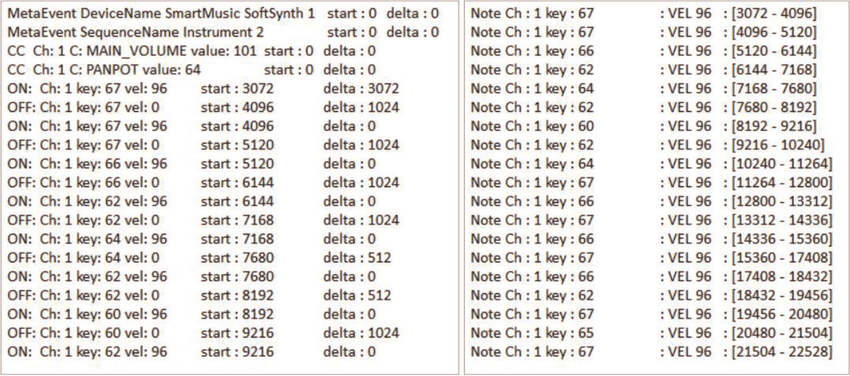
\includegraphics[scale=0.6, trim={0 0 13.8cm 0},clip]{figures/midi}
    \caption{Example MIDI arrangement in a readable format}
    \label{MIDIFigure}
\end{figure}

\subsection{Activation Functions}

In machine learning, the task of detecting instrument onsets could be described as a multi-label sequence labeling task. This involves, for each timeframe in a sequence, predicting a probability, or rather confidence value, that a certain instrument onset happens. In the domain of \gls{MIR} and \gls{AMT}, it has become common place to describe these confidence distributions as \textit{activation functions}; not to be confused with the general deep learning term, activation functions like ReLU or sigmoid.~\cite{8350302, Southall2016AutomaticDT, vogl2018multiinstrumentdrumtranscription}

This way of frame-level prediction is extensively used within onset detection in \gls{ADT} and is the approach we will be taking in this thesis. When predicting these activation functions, we concatenate each activation function distribution rowwise onto a matrix format, based on each instrument.

\begin{figure}[H]
    \centering
    \hspace*{-0.5cm}
    \begin{tikzpicture}

% Drum Sheet
\node[
    anchor=east,
    label=north:{\large{Drum Notation}}
] at (0, 0) {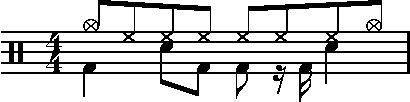
\includegraphics[scale=1.2]{lilypond/activations.cropped.pdf}};


% Activation Functions
\node[
    anchor=south
] at (5, 3.1) {\large{Activation Functions}};

% Cymbals and Ride
\draw[->,
thick
] (0, 0.5) -- (2, 2.5) node[midway, fill=white] {\acrshort{CC+RC}};
\draw[
    anchor=west,
    shift={(2.45, 2.1)}
] (-0.25, -0.1) -- (5.25, -0.1) -- (5.25, 0.9) -- (-0.25, 0.9) -- cycle;
\draw[
    anchor=west,
    color=blue,
    shift={(2.45, 2.1)}
] (-0.25, 0) -- (-0.05, 0) -- (0, 0.8) -- (0.05, 0) -- (4.95, 0) -- (5, 0.8) -- (5.05, 0) -- (5.25, 0);
\foreach \point in {(0, 0.8), (5, 0.8)} {
    \draw[
        color=red,
        shift={(2.45, 2.1)}
    ] \point circle (1.7pt);
}


% Hi-Hat
\draw[->,
thick
] (0, 0.25) -- (2, 1.25) node[midway, fill=white] {\acrshort{HH}};
\draw[
    line width=0.6pt,
    anchor=west,
    shift={(2.45, 0.85)}
] (-0.25, -0.1) -- (5.25, -0.1) -- (5.25, 0.9) -- (-0.25, 0.9) -- cycle;
\draw[
    anchor=west,
    color=blue,
    shift={(2.45, 0.85)}
] (-0.25, 0) -- (0.66, 0) -- (0.71, 0.8) -- (0.76, 0) -- (1.37, 0) -- (1.42, 0.8) -- (1.47, 0) -- (2.09, 0) -- (2.14, 0.8) -- (2.19, 0) -- (2.8, 0) -- (2.85, 0.8) -- (2.9, 0) -- (3.52, 0) -- (3.57, 0.8) -- (3.62, 0) -- (4.23, 0) -- (4.28, 0.8) -- (4.33, 0) -- (5.25, 0);
\foreach \point in {(0.71, 0.8), (1.42, 0.8), (2.14, 0.8), (2.85, 0.8), (3.57, 0.8), (4.28, 0.8)} {
    \draw[
        color=red,
        shift={(2.45, 0.85)}
    ] \point circle (1.7pt);
}


% Snare Drum
\draw[->,
thick
] (0, 0) -- (2, 0) node[midway, fill=white] {\acrshort{SD}};
\draw[
    anchor=west,
    shift={(2.45, -0.4)}
] (-0.25, -0.1) -- (5.25, -0.1) -- (5.25, 0.9) -- (-0.25, 0.9) -- cycle;
\draw[
    anchor=west,
    color=blue,
    shift={(2.45, -0.4)}
] (-0.25, 0) -- (1.37, 0) -- (1.42, 0.8) -- (1.47, 0) -- (4.23, 0) -- (4.28, 0.8) -- (4.33, 0) -- (5.25, 0);
\foreach \point in {(1.42, 0.8), (4.28, 0.8)} {
    \draw[
        color=red,
        shift={(2.45, -0.4)}
    ] \point circle (1.7pt);
}


% Tom-Toms
\draw[->,
thick
] (0, -0.25) -- (2, -1.25) node[midway, fill=white] {\acrshort{TT}};
\draw[
    anchor=west,
    shift={(2.45, -1.65)}
] (-0.25, -0.1) -- (5.25, -0.1) -- (5.25, 0.9) -- (-0.25, 0.9) -- cycle;
\draw[
    anchor=west,
    color=blue,
    shift={(2.45, -1.65)}
] (-0.25, 0) -- (5.25, 0);
\foreach \point in {} {
    \draw[
        color=red,
        shift={(2.45, -1.65)}
    ] \point circle (2pt);
}

% Kick Drum
\draw[->,
thick
] (0, -0.5) -- (2, -2.5) node[midway, fill=white] {\acrshort{KD}};
\draw[
    anchor=west,
    shift={(2.45, -2.9)}
] (-0.25, -0.1) -- (5.25, -0.1) -- (5.25, 0.9) -- (-0.25, 0.9) -- cycle;
\draw[
    anchor=west,
    color=blue,
    shift={(2.45, -2.9)}
] (-0.25, 0) -- (-0.05, 0) -- (0, 0.8) -- (0.05, 0) -- (2.09, 0) -- (2.14, 0.8) -- (2.19, 0) -- (2.8, 0) -- (2.85, 0.8) -- (2.9, 0) -- (3.87, 0) -- (3.92, 0.8) -- (3.97, 0) -- (5.25, 0);
\foreach \point in {(0, 0.8), (2.14, 0.8), (2.85, 0.8), (3.92, 0.8)} {
    \draw[
        color=red,
        shift={(2.45, -2.9)}
    ] \point circle (1.7pt);
}

\end{tikzpicture}
    \caption{The activation function representation for a 5-instrument \gls{ADT} task of a piece written in drum notation. Note how the value of each respective activation function is zero everywhere, except at its onsets, where it is one. The $\SePa$ symbol represents a short, 16th note rest in the \gls{KD} instrument, not an onset.}
    \label{ActivationsFigure}
\end{figure}

\subsubsection{Peak-picking}

When predicting activation functions, we need a separate post-processing step to turn these confidence distributions into onset events. By utilizing a standard \textit{peak-picking} algorithm, we can isolate and enhance peaks in these activation functions, and go from a continuous distribution to a collection of discrete events.

The peak-picking algorithm, introduced in its current form by Böck et al.~\cite{Bck2012EvaluatingTO}, defines that a prediction $\hat{y}_n$ at timeframe $n$ is a \textit{peak} if it fulfills the three conditions:
\begin{align*} 
    \hat{y}_n &= \text{max}(\hat{y}_{n - m}, ..., \hat{y}_n, ... \hat{y}_{n + m}), \\ 
    \hat{y}_n &\ge \text{mean}(\hat{y}_{n - a}, ..., \hat{y}_n, ... \hat{y}_{n + a}) + \delta, \\
    n &\ge n_\text{last onset} + w.
\end{align*}

For appropriately trained deep learning models, Vogl et al.~\cite{vogl2018multiinstrumentdrumtranscription} showed that the peak-picking parameters which gave the best results were $m = a = w = 2$ and $\delta = 0.1$. Consequently, these same parameter values are applied for this thesis.


\section{Automatic Drum Transcription}

\textcolor{red}{This whole section and the two other following need to be rewritten after moving them. Shouldn't be too big of an issue.}

As mentioned, \gls{ADT} describes the task of transcribing symbolic notation for drums from audio. To be even more descriptive, \gls{ADT} can be split into further tasks. From least to most complex we have: \gls{DSC}, where we classify drum instruments from isolated single event recordings. \gls{DTD}, where we transcribe audio containing exclusively drum instruments. \gls{DTP}, where we transcribe audio containing drum instruments, and additional percussive instruments which the transcription should exclude. Finally, we have \gls{DTM}, which describes the task of drum transcription with audio containing both drum, and melodic instruments.~\cite{8350302}

As mentioned, this thesis will focus on the most complex of these, namely \gls{DTM}. Intuitively, we want to develop a deep learning model which, given input audio, has the ability to detect and classify different drum instrument onsets (events), while selectively ignoring unrelated, melodic instruments.

This task comes with difficulties not seen in the less complex tasks. Zehren et al.~\cite{signals4040042} describes one example, in where \textit{"melodic and percussive instruments can overlap and mask eachother..., or have similar sounds, thus creating confusion between instruments"}.

Deep learning has shown to be a promising method to solve such a task, and several different approaches have been tried, many with great success. Vogl et al.~\cite{vogl2018multiinstrumentdrumtranscription, Vogl2017DrumTV} displayed good results with both a convolutional, and a convolutional-recurrent neural network. Zehren et al.~\cite{signals4040042, zehren2024analyzingreducingsynthetictorealtransfer} focused on datasets, showing that the amount of data and quality of data are equally important to get good performance. Most recently, Chang et al.~\cite{chang2024yourmt3+} explored an autoregressive, language model approach. This approach explored multi-instrument transcriptions, but their results regarding \gls{DTM} were notable.

This reinforces the fact that there still exist many approaches to attempt, which could lead to a general improvement for both general \gls{ADT} and \gls{DTM} models.

\section{The Drum Set}

The drum set is a collection of percussive instruments like different drums, cymbals, and possibly different auxillary percussions. A drum set can vary in what it is composed of, however a standard kit usually consists of a \gls{SD}, a \gls{KD}, one or more \glspl{TT} (toms), one or more cymbals (\gls{CC} and \gls{RC}), and a \gls{HH} cymbal~\cite{TheDrumHandbook2003}.

\begin{figure}[H]
    \centering
    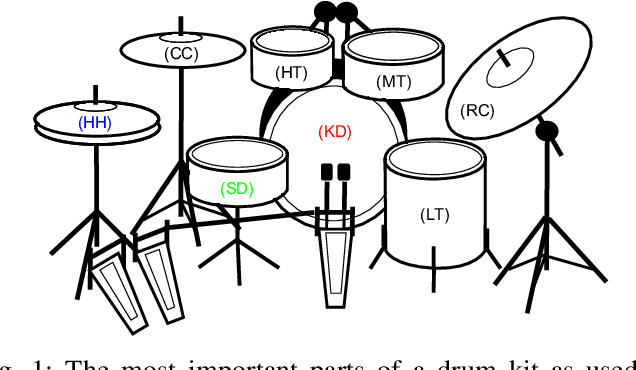
\includegraphics[scale=0.7, trim={0 1cm 0 0},clip]{figures/drumset}
    \caption{Example of the different instruments that make up the full standard drum set. They are the \acrfull{KD}, \acrfull{SD}, \acrfull{HH}, \acrfull{CC}, \acrfull{RC}, \acrfull{HT}, \acrfull{MT}, \acrfull{LT}.}
    \label{DrumsetFigure}
\end{figure}

As mentioned, percussion like the drum set, stands in contrast to other musical instruments in that the different ways of playing the same instrument often differ a lot in their \textit{"audible footprint"}. The snare drum, bass drum and hi-hat all have quite different timbres, frequency span, volume, and all in all fundamentally are different instruments.

\begin{figure}[H]
    \centering
    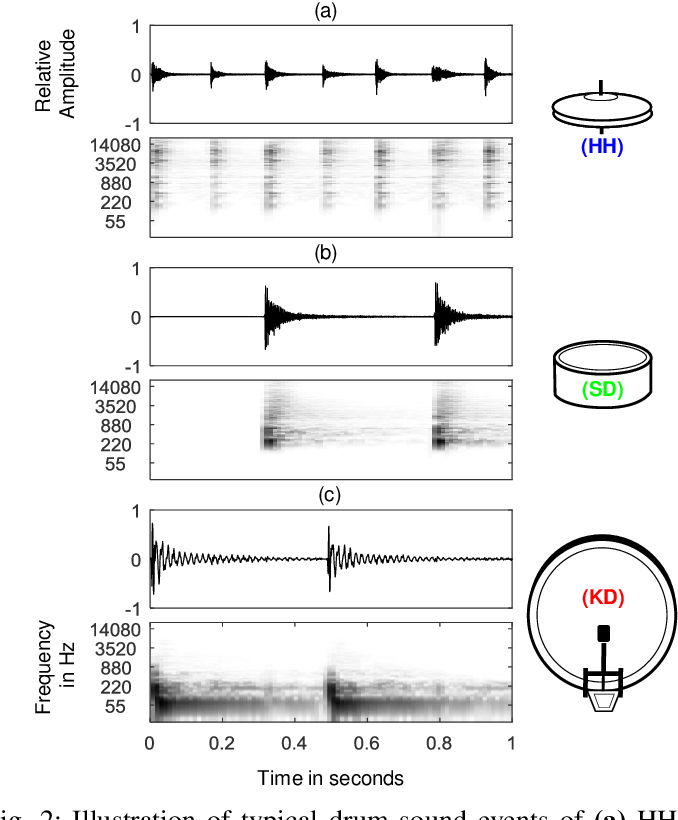
\includegraphics[scale=0.6, trim={0 1cm 0 0},clip]{figures/drumsettimbre}
    \caption{Example of the different audible footprint for drum set percussion. Plotted are the waveforms of three different drum instruments played at different speeds, together with its corresponding spectrogram. As we can see, each instrument event different significantly in how they look in and affect the spectrogram.}
    \label{DrumsetTimbreFigure}
\end{figure}

\section{Transcription Task}

Understand the pipeline for a transcription task, specifically \gls{ADT}, is crucial for this thesis. It all starts with an initial audio waveform representing the audio track we want to transcribe, usually split into smaller non-overlapping partitions~\cite{vogl2018multiinstrumentdrumtranscription, gardner2022mt3multitaskmultitrackmusic}. This is parsed into a spectrogram, which unravels the frequencies of the audio wave while condensing information across time, making the input features easier for a model to handle and interpret. The spectrogram is then input into an \gls{ADT} model, such as a \gls{DNN}, which reads this input spectrogram and for each timeframe predicts the probability that a certain instrument is played. These continuous likelihood predictions are then postprocessed into a more readable and intended format, such as drum notation.

\begin{figure}[H]
    \centering
    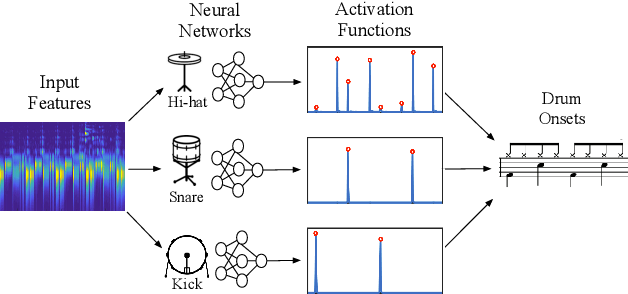
\includegraphics[scale=0.7]{figures/adtpipeline.png}
    \caption{Example of what the prediction pipeline of an \gls{ADT} model could look like. Given an input spectrogram, a model predicts a likelihood distribution of each instrument appearing (called the activation functions), which then is quantized into drum onsets and sheet music notation.}
    \label{ADTFigure}
\end{figure}

Following this pipeline there are certain parameters which need to be kept in mind when constructing the \gls{DNN}, namely: what does the input and ouput of model look like? The input is given as a spectrogram, but these can vary in size and format based different parameters. These will be discussed further in a later section. The output of the model has a sequence size based on the input spectrogram, but also based on the number of instruments we want to transcribe.

Early \gls{ADT} literature used a 3-instrument approach, predicting the basic \acrfull{KD}, \acrfull{SD} and \acrfull{HH}~\cite{vogl2016recurrent}. These give a useful basis in investigating wether \gls{ADT} problems are solvable using deep learning methods, but are too sparse as this leaves out instruments crucial to the basic drum set. To address this, we expand to a 5-instrument approach, including cymbals (capturing both \acrfull{CC} and \acrfull{RC}) and \acrfull{TT} (capturing all toms) in addition to the three prior instruments. This makes the problem slightly more complex, but allows for denser coverage by representing the standard, full drum set.


\section{Performance Measure}

\subsection{Correct Predictions}

Our machine learning models predict instrument onset events on a frame-level basis. In other words, are predictions are very granular, and we need some way to decide when a prediction is correct versus incorrect. In \gls{ADT}, a standard has become to allow a \textit{tolerance window} where event predictions are correct if they lie within a certain time window, often between $25\text{ms}$ and $50\text{ms}$. A side effect of this is that, by shifting our focus to predicted events, we lose information about \textit{not} predicting any events~\cite{vogl2016recurrent}.

\subsection{Accuracy}

For classification tasks, a standard performance measure would be \textit{accuracy}: \[ \text{Accuracy} = \frac{\text{TP} + \text{TN}}{\text{TP} + \text{TN} + \text{FP} + \text{FN}}.\] Summing up correct predictions, \gls{TP} and \gls{TN}, and dividing by total number of predictions, sum of \gls{TP}, \gls{TN}, \gls{FP} and \gls{FN}, we find a model's probability of having a correct prediction.

This performance measure falls short in that it is very susceptible to imbalanced datasets. In \gls{ADT}, most timeframes contain no onset, meaning a naïve predictor would get a high accuracy by never predicting any onsets. Another problem with accuracy is that, due to our tolerance window approach we do not necessarily have quantities for \gls{TN}, such that the standard accuracy computation would be incomputable.

\subsection{F1-score}

Mentioned above are some of the reasons why \textit{F1-score} has become the typical performance measure within \gls{ADT}. F1-score combines and tries to maximize two different performance measures, namely \textit{precision}; \[ \text{Precision} = \frac{\text{TP}}{\text{TP} + \text{FP}}, \] and \textit{recall}; \[ \text{Recall} = \frac{\text{TP}}{\text{TP} + \text{FN}}. \]

The precision of a model can tell us how good it is at \textit{hitting} predictions. \textit{Perfect precision} happens when a model has no \gls{FP}, i.e. never predicting an event where one doesn't happen. Recall is similar, but represents the other end of the stick. It tells us how good a model is at \textit{not missing} predictions. \textit{Perfect recall} happens when a model has no \gls{FN}, i.e. never \textit{not} predicting an event where one does happen.

As mentioned, F1-score combines these two measures in an aggregate performance measure by computing their harmonic mean: $$ \text{F1-score} = \frac{2 \cdot \text{Precision} \cdot \text{Recall}}{\text{Precision} + \text{Recall}}. $$ By maximizing F1, we simultaneously maximize both precision and recall as well, reaping all their benefits.

\subsection{Micro vs. Macro}

There are different ways of computing and combining F1-score on multi-label data. Even though they might seem similar, they fundamentally represent different information, and thus the choice in which one to select is crucial.

\textit{Macro F1-score} is computed through the arithmetic mean of the classwise computed F1-scores. Finding a model which maximizes this measure would be similar to finding the model which performes best on each of the separate classes, preventing a class from taking priority due to imbalanced datasets. Relating this to \gls{ADT}, it would mean focusing on transcribing each instrument equally well.

\textit{Micro F1-score} is computed through finding the F1-score with global \gls{TP}, \gls{FP}, \gls{FN} values. Maximizing this would mean prioritizing classes that occur more frequently in the datasets. Such as in \gls{ADT}, this would mean focusing on transcribing instruments which appear often, like the snare or base drum, over rarer instruments like the toms.

For \gls{ADT}, the trend has been to select Micro F1-score as the main performance measure, due to its ability to show a model's \textit{general} performance on musical pieces. We want our model to maximize their ability to transcribe music, not maximize their ability to transcribe each instrument in said music. \gls{ADT}, prioritizing frequent instruments is relevant. As mentioned previously, the more frequent instruments lay the ground work for the fundamentals, and could be said to be more important than scarcely occuring ones.

\begin{figure}[H]
    \centering
    \hspace*{-0.5cm}
    \begin{tikzpicture}
    
% True Transcription
\node[
    anchor=east,
    label=north:{\large{True Transcription}}
] (true) at (0, -0.5cm) {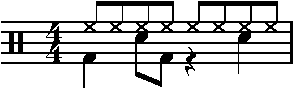
\includegraphics[scale=1.2]{lilypond/example_label.cropped.pdf}};

% Predicted Transcription
\node[
    anchor=west,
    label=north:{\large{Predicted Transcription}}
] (pred) at (0, -0.5cm) {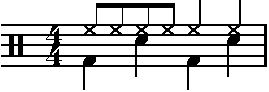
\includegraphics[scale=1.2]{lilypond/example_prediction.cropped.pdf}};


% False Positives
\node[
    anchor=north,
    label={[label distance=0.49cm]north:{\normalsize{\acrfullpl{FP}}}},
] (fp) at (0, -3cm) {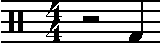
\includegraphics[scale=1.2]{lilypond/example_fp.cropped.pdf}};

% True Positives
\node[
    anchor=north,
    label=north:{\normalsize{\acrfullpl{TP}}},
    left=0.25cm of fp
] {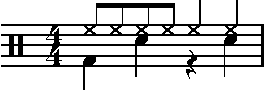
\includegraphics[scale=1.2]{lilypond/example_tp.cropped.pdf}};
    
% False Negatives
\node[
    anchor=north,
    label={[label distance=0.49cm]north:{\normalsize{\acrfullpl{FN}}}},
    right=0.25cm of fp
] {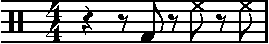
\includegraphics[scale=1.2]{lilypond/example_fn.cropped.pdf}};

\matrix[
    column sep=0.5cm
] at (0, -5cm) {
    \node {\large{\textbf{Classwise F1}:}}; &
    \node[
        label=north:{\large{\acrshort{KD}}}
    ] {\large{0.5}}; &
    \node[
        label=north:{\large{\acrshort{SD}}}
    ] {\large{1.0}}; &
    \node[
        label=north:{\large{\acrshort{HH}}}
    ]{\large{0.86}}; \\
};
\matrix[
    column sep=0.5cm
] at (0, -6cm) {
    \node {\large{\textbf{Macro F1}: 0.79}}; &
    \node {\large{\textbf{Micro F1}: 0.82}}; \\
};


\end{tikzpicture}
    \caption{Example of computing the different F1-scores of from a true and predicted \gls{ADT} transcription. The \HaPa, \ViPa, or \AcPa symbols represent pauses, and not instrument onsets. Note how the Macro F1 better represents the F1-score of all individual instruments, where as Micro F1 better represents the F1-score of the transcription as a whole. For readability, F1-scores are written with a precision of two decimals.}
    \label{F1Figure}
\end{figure}